\documentclass[10pt]{article}
\usepackage[margin=1.0cm]{geometry}
\usepackage[T1]{fontenc}
\usepackage{lmodern}
\usepackage{xcolor}
\usepackage{tikz}
\usepackage{pgfplots}
\usepgfplotslibrary{statistics}
\pgfplotsset{compat=1.18}
\definecolor{srblue}{HTML}{2F6B9A}
\definecolor{opencvorange}{HTML}{D97706}
\definecolor{fps2blue}{HTML}{B9D7EA}
\definecolor{fps5orange}{HTML}{F6C28B}
\definecolor{stslightgreen}{HTML}{A7D8B1}
\definecolor{stsstronggreen}{HTML}{208B3A}
\definecolor{sugarlightpurple}{HTML}{CBB7E8}
\definecolor{sugarstrongpurple}{HTML}{763A9B}
\definecolor{stsedge}{HTML}{1D4E89}
\definecolor{sugaredge}{HTML}{B45309}
\definecolor{incompletegray}{HTML}{9CA3AF}
\definecolor{deltared}{HTML}{B91C1C}
\definecolor{deltagreen}{HTML}{15803D}
\begin{document}
\pagestyle{empty}
\begin{center}
{\Large\bfseries Gemittelte Bildmetriken im Verhältnis zur Laufzeit}\\[3pt]
{\small Mittelwerte aus historischen und Repeat-Läufen}\\[8pt]
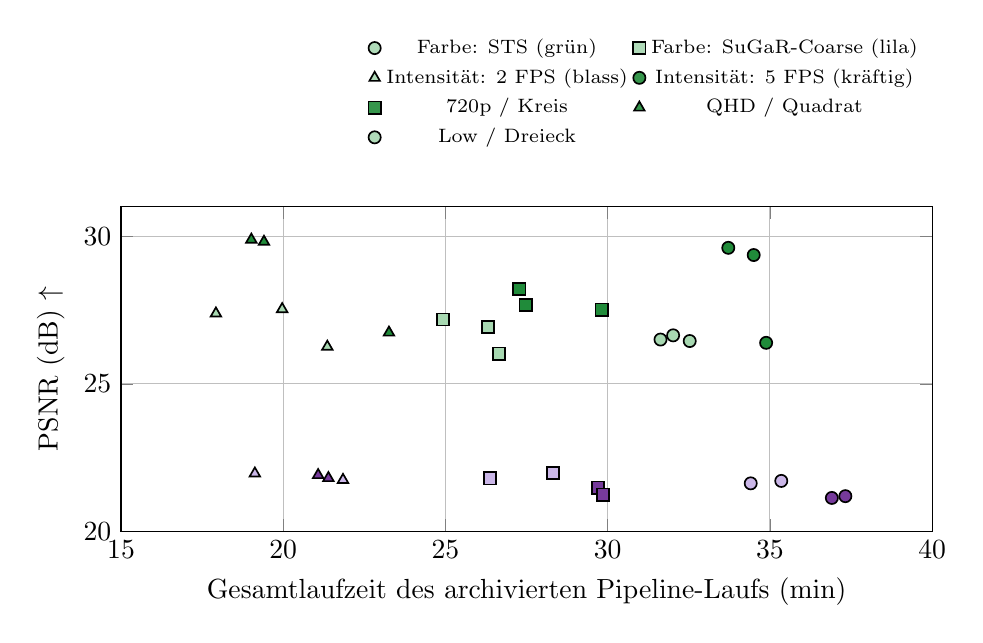
\begin{tikzpicture}
\begin{axis}[width=0.98\linewidth,height=5.7cm,xlabel={Gesamtlaufzeit des archivierten Pipeline-Laufs (min)},ylabel={PSNR (dB) $\uparrow$},xmin=15,xmax=40,xtick={15,20,25,30,35,40},ymin=20,ymax=31,grid=major,legend style={font=\scriptsize,at={(1.0,1.15)},anchor=south east,draw=none,fill=white,fill opacity=0.9,text opacity=1},legend columns=2]
\addplot[only marks,mark=*,mark size=2.2pt,mark options={fill=stslightgreen,draw=black,line width=0.6pt}] coordinates {(31.627778,26.50121269)};
\addplot[only marks,mark=square*,mark size=2.2pt,mark options={fill=stslightgreen,draw=black,line width=0.6pt}] coordinates {(24.925000,27.18327996)};
\addplot[only marks,mark=triangle*,mark size=2.2pt,mark options={fill=stslightgreen,draw=black,line width=0.6pt}] coordinates {(17.925000,27.38534741)};
\addplot[only marks,mark=*,mark size=2.2pt,mark options={fill=stsstronggreen,draw=black,line width=0.6pt}] coordinates {(34.500000,29.36834851)};
\addplot[only marks,mark=square*,mark size=2.2pt,mark options={fill=stsstronggreen,draw=black,line width=0.6pt}] coordinates {(27.277778,28.20878513)};
\addplot[only marks,mark=triangle*,mark size=2.2pt,mark options={fill=stsstronggreen,draw=black,line width=0.6pt}] coordinates {(19.405556,29.81829738)};
\addplot[only marks,mark=*,mark size=2.2pt,mark options={fill=stslightgreen,draw=black,line width=0.6pt}] coordinates {(32.527778,26.45132990)};
\addplot[only marks,mark=square*,mark size=2.2pt,mark options={fill=stslightgreen,draw=black,line width=0.6pt}] coordinates {(26.316667,26.91983874)};
\addplot[only marks,mark=triangle*,mark size=2.2pt,mark options={fill=stslightgreen,draw=black,line width=0.6pt}] coordinates {(19.966667,27.53341959)};
\addplot[only marks,mark=*,mark size=2.2pt,mark options={fill=stsstronggreen,draw=black,line width=0.6pt}] coordinates {(33.716667,29.61294152)};
\addplot[only marks,mark=square*,mark size=2.2pt,mark options={fill=stsstronggreen,draw=black,line width=0.6pt}] coordinates {(27.472222,27.66550179)};
\addplot[only marks,mark=triangle*,mark size=2.2pt,mark options={fill=stsstronggreen,draw=black,line width=0.6pt}] coordinates {(19.016667,29.89049716)};
\addplot[only marks,mark=*,mark size=2.2pt,mark options={fill=stslightgreen,draw=black,line width=0.6pt}] coordinates {(32.016667,26.64421298)};
\addplot[only marks,mark=square*,mark size=2.2pt,mark options={fill=stslightgreen,draw=black,line width=0.6pt}] coordinates {(26.650000,26.02053897)};
\addplot[only marks,mark=triangle*,mark size=2.2pt,mark options={fill=stslightgreen,draw=black,line width=0.6pt}] coordinates {(21.358333,26.25806929)};
\addplot[only marks,mark=*,mark size=2.2pt,mark options={fill=stsstronggreen,draw=black,line width=0.6pt}] coordinates {(34.883333,26.39010134)};
\addplot[only marks,mark=square*,mark size=2.2pt,mark options={fill=stsstronggreen,draw=black,line width=0.6pt}] coordinates {(29.816667,27.51721004)};
\addplot[only marks,mark=triangle*,mark size=2.2pt,mark options={fill=stsstronggreen,draw=black,line width=0.6pt}] coordinates {(23.258333,26.73754651)};
\addplot[only marks,mark=*,mark size=2.2pt,mark options={fill=sugarlightpurple,draw=black,line width=0.6pt}] coordinates {(34.408333,21.62396527)};
\addplot[only marks,mark=square*,mark size=2.2pt,mark options={fill=sugarlightpurple,draw=black,line width=0.6pt}] coordinates {(26.366667,21.79592392)};
\addplot[only marks,mark=triangle*,mark size=2.2pt,mark options={fill=sugarlightpurple,draw=black,line width=0.6pt}] coordinates {(19.125000,21.95754552)};
\addplot[only marks,mark=*,mark size=2.2pt,mark options={fill=sugarstrongpurple,draw=black,line width=0.6pt}] coordinates {(37.325000,21.18935272)};
\addplot[only marks,mark=square*,mark size=2.2pt,mark options={fill=sugarstrongpurple,draw=black,line width=0.6pt}] coordinates {(29.700000,21.47751191)};
\addplot[only marks,mark=triangle*,mark size=2.2pt,mark options={fill=sugarstrongpurple,draw=black,line width=0.6pt}] coordinates {(21.391667,21.80319613)};
\addplot[only marks,mark=*,mark size=2.2pt,mark options={fill=sugarlightpurple,draw=black,line width=0.6pt}] coordinates {(35.350000,21.70630497)};
\addplot[only marks,mark=square*,mark size=2.2pt,mark options={fill=sugarlightpurple,draw=black,line width=0.6pt}] coordinates {(28.316667,21.98231481)};
\addplot[only marks,mark=triangle*,mark size=2.2pt,mark options={fill=sugarlightpurple,draw=black,line width=0.6pt}] coordinates {(21.841667,21.74027143)};
\addplot[only marks,mark=*,mark size=2.2pt,mark options={fill=sugarstrongpurple,draw=black,line width=0.6pt}] coordinates {(36.908333,21.12920408)};
\addplot[only marks,mark=square*,mark size=2.2pt,mark options={fill=sugarstrongpurple,draw=black,line width=0.6pt}] coordinates {(29.850000,21.23772442)};
\addplot[only marks,mark=triangle*,mark size=2.2pt,mark options={fill=sugarstrongpurple,draw=black,line width=0.6pt}] coordinates {(21.075000,21.90462963)};
\addlegendimage{only marks,mark=*,mark size=2.2pt,mark options={fill=stsstronggreen,draw=black}}\addlegendentry{Farbe: STS (grün)}
\addlegendimage{only marks,mark=*,mark size=2.2pt,mark options={fill=sugarstrongpurple,draw=black}}\addlegendentry{Farbe: SuGaR-Coarse (lila)}
\addlegendimage{only marks,mark=*,mark size=2.2pt,mark options={fill=stslightgreen,draw=black}}\addlegendentry{Intensität: 2 FPS (blass)}
\addlegendimage{only marks,mark=*,mark size=2.2pt,mark options={fill=stsstronggreen,draw=black}}\addlegendentry{Intensität: 5 FPS (kräftig)}
\addlegendimage{only marks,mark=*,mark size=2.2pt,mark options={fill=white,draw=black}}\addlegendentry{720p / Kreis}
\addlegendimage{only marks,mark=square*,mark size=2.2pt,mark options={fill=white,draw=black}}\addlegendentry{QHD / Quadrat}
\addlegendimage{only marks,mark=triangle*,mark size=2.2pt,mark options={fill=white,draw=black}}\addlegendentry{Low / Dreieck}
\end{axis}\end{tikzpicture}\par\vspace{2pt}
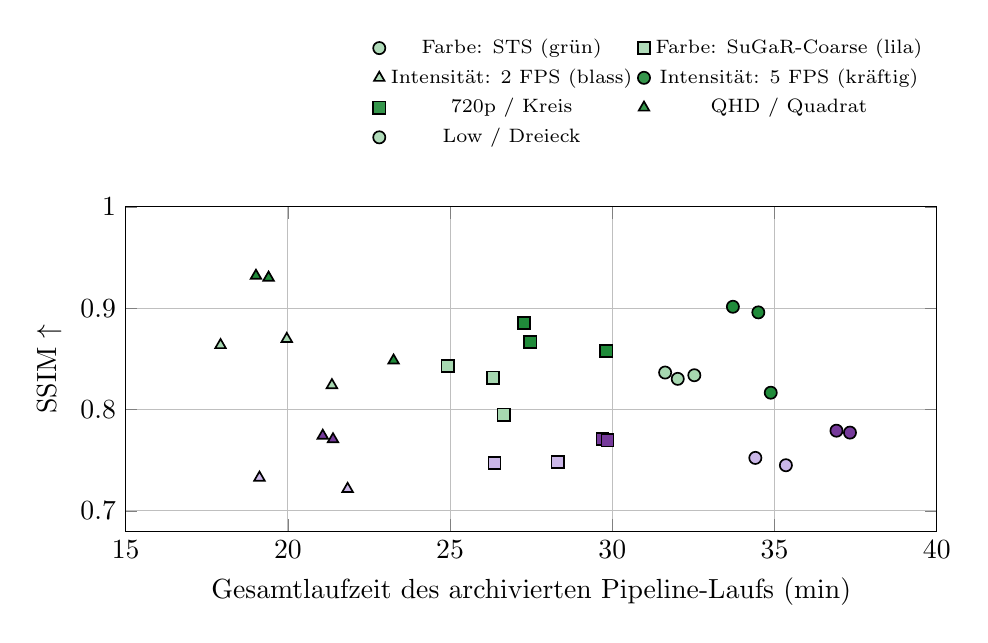
\begin{tikzpicture}
\begin{axis}[width=0.98\linewidth,height=5.7cm,xlabel={Gesamtlaufzeit des archivierten Pipeline-Laufs (min)},ylabel={SSIM $\uparrow$},xmin=15,xmax=40,xtick={15,20,25,30,35,40},ymin=0.68,ymax=1.0,grid=major,legend style={font=\scriptsize,at={(1.0,1.15)},anchor=south east,draw=none,fill=white,fill opacity=0.9,text opacity=1},legend columns=2]
\addplot[only marks,mark=*,mark size=2.2pt,mark options={fill=stslightgreen,draw=black,line width=0.6pt}] coordinates {(31.627778,0.83657259)};
\addplot[only marks,mark=square*,mark size=2.2pt,mark options={fill=stslightgreen,draw=black,line width=0.6pt}] coordinates {(24.925000,0.84303451)};
\addplot[only marks,mark=triangle*,mark size=2.2pt,mark options={fill=stslightgreen,draw=black,line width=0.6pt}] coordinates {(17.925000,0.86367902)};
\addplot[only marks,mark=*,mark size=2.2pt,mark options={fill=stsstronggreen,draw=black,line width=0.6pt}] coordinates {(34.500000,0.89594813)};
\addplot[only marks,mark=square*,mark size=2.2pt,mark options={fill=stsstronggreen,draw=black,line width=0.6pt}] coordinates {(27.277778,0.88555103)};
\addplot[only marks,mark=triangle*,mark size=2.2pt,mark options={fill=stsstronggreen,draw=black,line width=0.6pt}] coordinates {(19.405556,0.93023792)};
\addplot[only marks,mark=*,mark size=2.2pt,mark options={fill=stslightgreen,draw=black,line width=0.6pt}] coordinates {(32.527778,0.83392095)};
\addplot[only marks,mark=square*,mark size=2.2pt,mark options={fill=stslightgreen,draw=black,line width=0.6pt}] coordinates {(26.316667,0.83151061)};
\addplot[only marks,mark=triangle*,mark size=2.2pt,mark options={fill=stslightgreen,draw=black,line width=0.6pt}] coordinates {(19.966667,0.86978696)};
\addplot[only marks,mark=*,mark size=2.2pt,mark options={fill=stsstronggreen,draw=black,line width=0.6pt}] coordinates {(33.716667,0.90148111)};
\addplot[only marks,mark=square*,mark size=2.2pt,mark options={fill=stsstronggreen,draw=black,line width=0.6pt}] coordinates {(27.472222,0.86666241)};
\addplot[only marks,mark=triangle*,mark size=2.2pt,mark options={fill=stsstronggreen,draw=black,line width=0.6pt}] coordinates {(19.016667,0.93208752)};
\addplot[only marks,mark=*,mark size=2.2pt,mark options={fill=stslightgreen,draw=black,line width=0.6pt}] coordinates {(32.016667,0.83034673)};
\addplot[only marks,mark=square*,mark size=2.2pt,mark options={fill=stslightgreen,draw=black,line width=0.6pt}] coordinates {(26.650000,0.79501773)};
\addplot[only marks,mark=triangle*,mark size=2.2pt,mark options={fill=stslightgreen,draw=black,line width=0.6pt}] coordinates {(21.358333,0.82414792)};
\addplot[only marks,mark=*,mark size=2.2pt,mark options={fill=stsstronggreen,draw=black,line width=0.6pt}] coordinates {(34.883333,0.81667582)};
\addplot[only marks,mark=square*,mark size=2.2pt,mark options={fill=stsstronggreen,draw=black,line width=0.6pt}] coordinates {(29.816667,0.85779472)};
\addplot[only marks,mark=triangle*,mark size=2.2pt,mark options={fill=stsstronggreen,draw=black,line width=0.6pt}] coordinates {(23.258333,0.84843206)};
\addplot[only marks,mark=*,mark size=2.2pt,mark options={fill=sugarlightpurple,draw=black,line width=0.6pt}] coordinates {(34.408333,0.75235156)};
\addplot[only marks,mark=square*,mark size=2.2pt,mark options={fill=sugarlightpurple,draw=black,line width=0.6pt}] coordinates {(26.366667,0.74728784)};
\addplot[only marks,mark=triangle*,mark size=2.2pt,mark options={fill=sugarlightpurple,draw=black,line width=0.6pt}] coordinates {(19.125000,0.73286190)};
\addplot[only marks,mark=*,mark size=2.2pt,mark options={fill=sugarstrongpurple,draw=black,line width=0.6pt}] coordinates {(37.325000,0.77730088)};
\addplot[only marks,mark=square*,mark size=2.2pt,mark options={fill=sugarstrongpurple,draw=black,line width=0.6pt}] coordinates {(29.700000,0.77080612)};
\addplot[only marks,mark=triangle*,mark size=2.2pt,mark options={fill=sugarstrongpurple,draw=black,line width=0.6pt}] coordinates {(21.391667,0.77073706)};
\addplot[only marks,mark=*,mark size=2.2pt,mark options={fill=sugarlightpurple,draw=black,line width=0.6pt}] coordinates {(35.350000,0.74509775)};
\addplot[only marks,mark=square*,mark size=2.2pt,mark options={fill=sugarlightpurple,draw=black,line width=0.6pt}] coordinates {(28.316667,0.74816444)};
\addplot[only marks,mark=triangle*,mark size=2.2pt,mark options={fill=sugarlightpurple,draw=black,line width=0.6pt}] coordinates {(21.841667,0.72177499)};
\addplot[only marks,mark=*,mark size=2.2pt,mark options={fill=sugarstrongpurple,draw=black,line width=0.6pt}] coordinates {(36.908333,0.77919533)};
\addplot[only marks,mark=square*,mark size=2.2pt,mark options={fill=sugarstrongpurple,draw=black,line width=0.6pt}] coordinates {(29.850000,0.76970694)};
\addplot[only marks,mark=triangle*,mark size=2.2pt,mark options={fill=sugarstrongpurple,draw=black,line width=0.6pt}] coordinates {(21.075000,0.77422207)};
\addlegendimage{only marks,mark=*,mark size=2.2pt,mark options={fill=stsstronggreen,draw=black}}\addlegendentry{Farbe: STS (grün)}
\addlegendimage{only marks,mark=*,mark size=2.2pt,mark options={fill=sugarstrongpurple,draw=black}}\addlegendentry{Farbe: SuGaR-Coarse (lila)}
\addlegendimage{only marks,mark=*,mark size=2.2pt,mark options={fill=stslightgreen,draw=black}}\addlegendentry{Intensität: 2 FPS (blass)}
\addlegendimage{only marks,mark=*,mark size=2.2pt,mark options={fill=stsstronggreen,draw=black}}\addlegendentry{Intensität: 5 FPS (kräftig)}
\addlegendimage{only marks,mark=*,mark size=2.2pt,mark options={fill=white,draw=black}}\addlegendentry{720p / Kreis}
\addlegendimage{only marks,mark=square*,mark size=2.2pt,mark options={fill=white,draw=black}}\addlegendentry{QHD / Quadrat}
\addlegendimage{only marks,mark=triangle*,mark size=2.2pt,mark options={fill=white,draw=black}}\addlegendentry{Low / Dreieck}
\end{axis}\end{tikzpicture}\par\vspace{2pt}
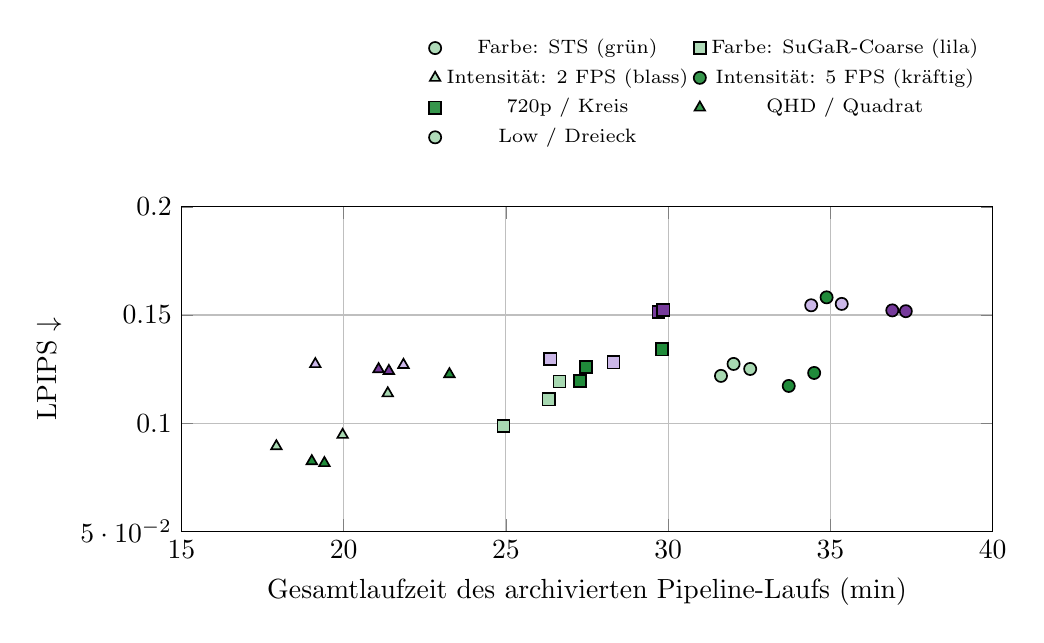
\begin{tikzpicture}
\begin{axis}[width=0.98\linewidth,height=5.7cm,xlabel={Gesamtlaufzeit des archivierten Pipeline-Laufs (min)},ylabel={LPIPS $\downarrow$},xmin=15,xmax=40,xtick={15,20,25,30,35,40},ymin=0.05,ymax=0.2,grid=major,legend style={font=\scriptsize,at={(1.0,1.15)},anchor=south east,draw=none,fill=white,fill opacity=0.9,text opacity=1},legend columns=2]
\addplot[only marks,mark=*,mark size=2.2pt,mark options={fill=stslightgreen,draw=black,line width=0.6pt}] coordinates {(31.627778,0.12185202)};
\addplot[only marks,mark=square*,mark size=2.2pt,mark options={fill=stslightgreen,draw=black,line width=0.6pt}] coordinates {(24.925000,0.09865326)};
\addplot[only marks,mark=triangle*,mark size=2.2pt,mark options={fill=stslightgreen,draw=black,line width=0.6pt}] coordinates {(17.925000,0.08929665)};
\addplot[only marks,mark=*,mark size=2.2pt,mark options={fill=stsstronggreen,draw=black,line width=0.6pt}] coordinates {(34.500000,0.12320841)};
\addplot[only marks,mark=square*,mark size=2.2pt,mark options={fill=stsstronggreen,draw=black,line width=0.6pt}] coordinates {(27.277778,0.11937699)};
\addplot[only marks,mark=triangle*,mark size=2.2pt,mark options={fill=stsstronggreen,draw=black,line width=0.6pt}] coordinates {(19.405556,0.08152318)};
\addplot[only marks,mark=*,mark size=2.2pt,mark options={fill=stslightgreen,draw=black,line width=0.6pt}] coordinates {(32.527778,0.12505824)};
\addplot[only marks,mark=square*,mark size=2.2pt,mark options={fill=stslightgreen,draw=black,line width=0.6pt}] coordinates {(26.316667,0.11104393)};
\addplot[only marks,mark=triangle*,mark size=2.2pt,mark options={fill=stslightgreen,draw=black,line width=0.6pt}] coordinates {(19.966667,0.09456848)};
\addplot[only marks,mark=*,mark size=2.2pt,mark options={fill=stsstronggreen,draw=black,line width=0.6pt}] coordinates {(33.716667,0.11720216)};
\addplot[only marks,mark=square*,mark size=2.2pt,mark options={fill=stsstronggreen,draw=black,line width=0.6pt}] coordinates {(27.472222,0.12601008)};
\addplot[only marks,mark=triangle*,mark size=2.2pt,mark options={fill=stsstronggreen,draw=black,line width=0.6pt}] coordinates {(19.016667,0.08239057)};
\addplot[only marks,mark=*,mark size=2.2pt,mark options={fill=stslightgreen,draw=black,line width=0.6pt}] coordinates {(32.016667,0.12737379)};
\addplot[only marks,mark=square*,mark size=2.2pt,mark options={fill=stslightgreen,draw=black,line width=0.6pt}] coordinates {(26.650000,0.11923454)};
\addplot[only marks,mark=triangle*,mark size=2.2pt,mark options={fill=stslightgreen,draw=black,line width=0.6pt}] coordinates {(21.358333,0.11378294)};
\addplot[only marks,mark=*,mark size=2.2pt,mark options={fill=stsstronggreen,draw=black,line width=0.6pt}] coordinates {(34.883333,0.15818454)};
\addplot[only marks,mark=square*,mark size=2.2pt,mark options={fill=stsstronggreen,draw=black,line width=0.6pt}] coordinates {(29.816667,0.13414868)};
\addplot[only marks,mark=triangle*,mark size=2.2pt,mark options={fill=stsstronggreen,draw=black,line width=0.6pt}] coordinates {(23.258333,0.12262199)};
\addplot[only marks,mark=*,mark size=2.2pt,mark options={fill=sugarlightpurple,draw=black,line width=0.6pt}] coordinates {(34.408333,0.15450558)};
\addplot[only marks,mark=square*,mark size=2.2pt,mark options={fill=sugarlightpurple,draw=black,line width=0.6pt}] coordinates {(26.366667,0.12963476)};
\addplot[only marks,mark=triangle*,mark size=2.2pt,mark options={fill=sugarlightpurple,draw=black,line width=0.6pt}] coordinates {(19.125000,0.12729331)};
\addplot[only marks,mark=*,mark size=2.2pt,mark options={fill=sugarstrongpurple,draw=black,line width=0.6pt}] coordinates {(37.325000,0.15177572)};
\addplot[only marks,mark=square*,mark size=2.2pt,mark options={fill=sugarstrongpurple,draw=black,line width=0.6pt}] coordinates {(29.700000,0.15147646)};
\addplot[only marks,mark=triangle*,mark size=2.2pt,mark options={fill=sugarstrongpurple,draw=black,line width=0.6pt}] coordinates {(21.391667,0.12412121)};
\addplot[only marks,mark=*,mark size=2.2pt,mark options={fill=sugarlightpurple,draw=black,line width=0.6pt}] coordinates {(35.350000,0.15514735)};
\addplot[only marks,mark=square*,mark size=2.2pt,mark options={fill=sugarlightpurple,draw=black,line width=0.6pt}] coordinates {(28.316667,0.12811350)};
\addplot[only marks,mark=triangle*,mark size=2.2pt,mark options={fill=sugarlightpurple,draw=black,line width=0.6pt}] coordinates {(21.841667,0.12693911)};
\addplot[only marks,mark=*,mark size=2.2pt,mark options={fill=sugarstrongpurple,draw=black,line width=0.6pt}] coordinates {(36.908333,0.15214804)};
\addplot[only marks,mark=square*,mark size=2.2pt,mark options={fill=sugarstrongpurple,draw=black,line width=0.6pt}] coordinates {(29.850000,0.15238602)};
\addplot[only marks,mark=triangle*,mark size=2.2pt,mark options={fill=sugarstrongpurple,draw=black,line width=0.6pt}] coordinates {(21.075000,0.12494864)};
\addlegendimage{only marks,mark=*,mark size=2.2pt,mark options={fill=stsstronggreen,draw=black}}\addlegendentry{Farbe: STS (grün)}
\addlegendimage{only marks,mark=*,mark size=2.2pt,mark options={fill=sugarstrongpurple,draw=black}}\addlegendentry{Farbe: SuGaR-Coarse (lila)}
\addlegendimage{only marks,mark=*,mark size=2.2pt,mark options={fill=stslightgreen,draw=black}}\addlegendentry{Intensität: 2 FPS (blass)}
\addlegendimage{only marks,mark=*,mark size=2.2pt,mark options={fill=stsstronggreen,draw=black}}\addlegendentry{Intensität: 5 FPS (kräftig)}
\addlegendimage{only marks,mark=*,mark size=2.2pt,mark options={fill=white,draw=black}}\addlegendentry{720p / Kreis}
\addlegendimage{only marks,mark=square*,mark size=2.2pt,mark options={fill=white,draw=black}}\addlegendentry{QHD / Quadrat}
\addlegendimage{only marks,mark=triangle*,mark size=2.2pt,mark options={fill=white,draw=black}}\addlegendentry{Low / Dreieck}
\end{axis}\end{tikzpicture}\par\vspace{2pt}
\vspace{3pt}
\begin{minipage}{0.98\linewidth}\scriptsize Die x-Achse zeigt die vollständige Dauer des archivierten Pipeline-Laufs zwischen Start und Ende in \texttt{run.md}; ältere Berichte ohne Start/Ende verwenden ersatzweise die Summe ihrer aufgezeichneten Schritte. SAM3/COLMAP sind nur enthalten, sofern sie innerhalb dieses archivierten Laufs lagen. Die Darstellung ist explorativ und kein Geometrie-Qualitätsranking.\end{minipage}
\end{center}
\end{document}